{\color{blue}{
\subsection{{\bf Comparison on Name Prediction (JS)}}
\label{empirical-rq1}

\begin{figure}[t] %[thbp]
\begin{center}
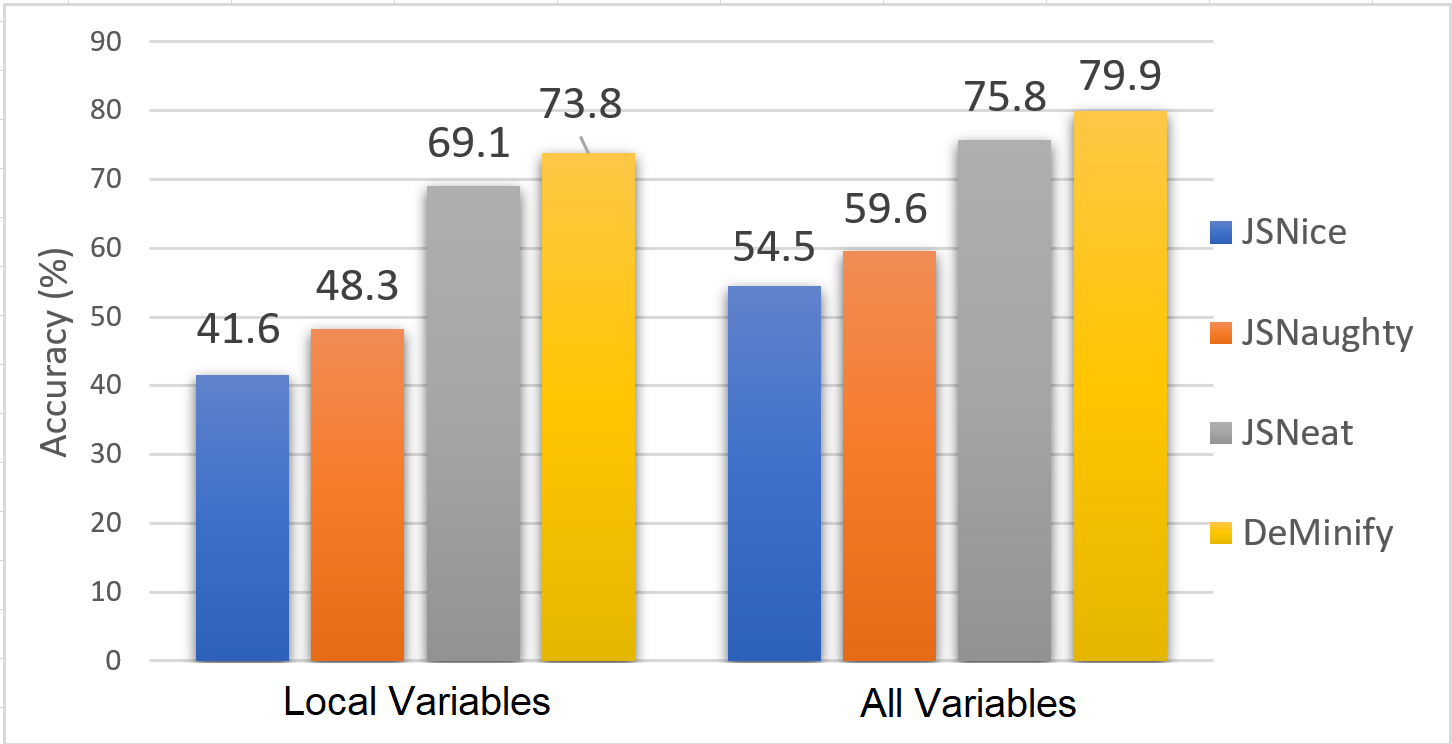
\includegraphics[width=3.2in]{figures/name-JS-prediction-result}
\vspace{-8pt}
\caption{{\color{blue}{RQ2. Top-1 Accuracy on Name Prediction (JS)}}}
\label{name-JS-prediction-result}
\end{center}
\end{figure}

As seen in Figure~\ref{name-JS-prediction-result}, for all variables in
minified code, {\tool} achieves high top-1 accuracy of {\bf 79.9\%}:
in almost 4 out 5 cases, it can recover the correct variable names with
a single prediction. The relative improvements in top-1 accuracy for
all variables over JSNice, JSNaughty, and JSNeat are {\bf 46.6\%,
  34.0\%}, and {\bf 5.4\%}, respectively.
The absolute improvements in top-1 accuracy over the state-of-the-art
approaches are from 4.1\%--25.4\%.

Considering only local variables, in {\bf 73.8\%} of them, {\tool}
correctly predicts their original names with a single result. The
relative improvements in top-1 accuracy in recovering local variables'
names over JSNice, JSNaughty, and JSNeat are {\bf 77.4\%, 52.7\%}, and
{\bf 6.8\%}, respectively. The absolute improvements in top-1
accuracy over the state-of-the-art approaches are from 4.7\%--32.2\%.

\begin{table}[t]%[thbp]
  \caption{{\color{blue}{RQ2. Comparison on Name Prediction (JS)}}}
  \vspace{-8pt}
	\begin{center}
		\small
		\renewcommand{\arraystretch}{1} \begin{tabular}{|p{1.9cm}<{\centering}|p{0.65cm}<{\centering}|p{0.65cm}<{\centering}|p{0.65cm}<{\centering}|p{0.65cm}<{\centering}|p{0.65cm}<{\centering}|p{0.65cm}<{\centering}|}
			
			\hline
                       & \multicolumn{2}{c|}{Top-1}         & \multicolumn{2}{c|}{Top-3}         & \multicolumn{2}{c|}{Top-5} \\
			\hline
                       & Local & All & Local & All & Local & All  \\ 
			\hline
		        JSNice~\cite{JSNice2015} &  41.6    & 54.5  & 56.4 &    68.2   & 64.2      &   72.4    \\
			JSNaughty~\cite{JSNaughty2017}  &   48.3   &  59.6    &  64.1    &  74.5    &  71.8    &   79.6    \\
			JSNeat~\cite{icse19}  &   69.1   &  75.8    &  69.6    & 79.5     &  76.9    & 86.0     \\
			\hline
			{\bf {\tool}} & 73.8 & 79.9 & 79.2 & 89.6 & 87.3 & 96.8 \\
			\hline
		\end{tabular}
		\label{name-JS-result}
	\end{center}
\end{table}

%Tien

As seen in Figures~\ref{name-prediction-result}
and~\ref{name-JS-prediction-result}, the results are consistent for
both languages. However, the relative improvement of {\tool} over the
top baseline, JSNeat, for Python is higher than that for JS. The
reason is that JSNeat, an IR approach, was able to find more variable
names in the JS dataset than in the Python dataset.  Note that JSNeat
was built on JS code. Moreover, there are less variable names that
need predictions in JS dataset than in Python dataset.


}}
